\section{Hardware}

\subsection{Schmetic}
\begin{figure}[H]
	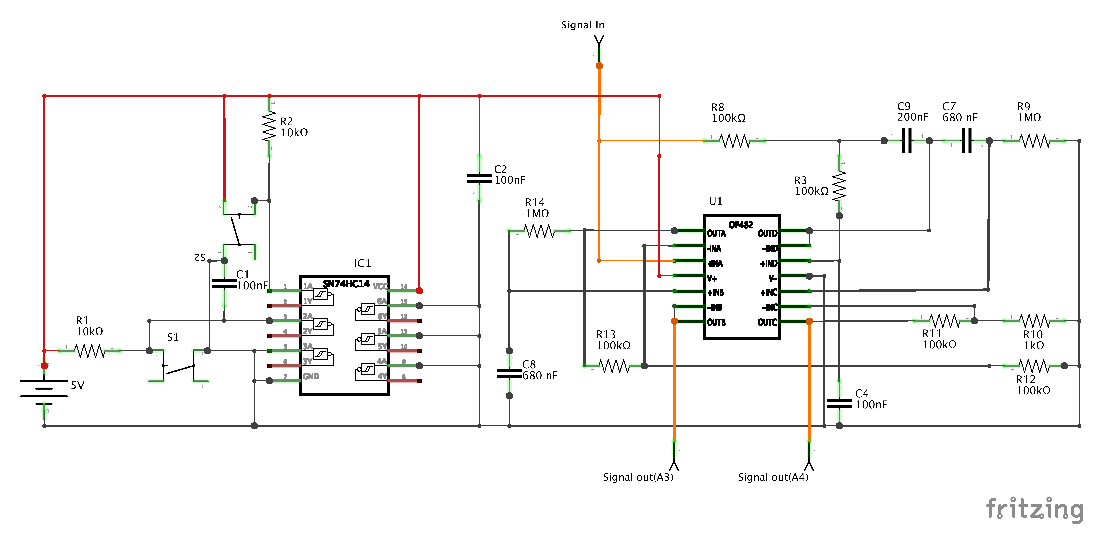
\includegraphics[trim = 0 30 0 0, clip=true, width = \textwidth]{billeder/Konditionering_schem.pdf}
	\caption{}\label{fig:schematics}
\end{figure}

\subsection{Knapper} \label{title:buttons}
For at imødegå debouncing ved tryk på knapperne, er der bygget et støttekredsløbs til disse. Debouning kan ses på figur \ref{fig:withbounce} hvor det mekaniske splip på knappen, giver anledning til en løs forbindelse ses på multimeteret som en lav efterfulgt af en høj, for så at blive lav igen. Microcontrolleren er hurtig nok til at registrer dette som et nyt knaptryk.
\begin{figure}[H]
	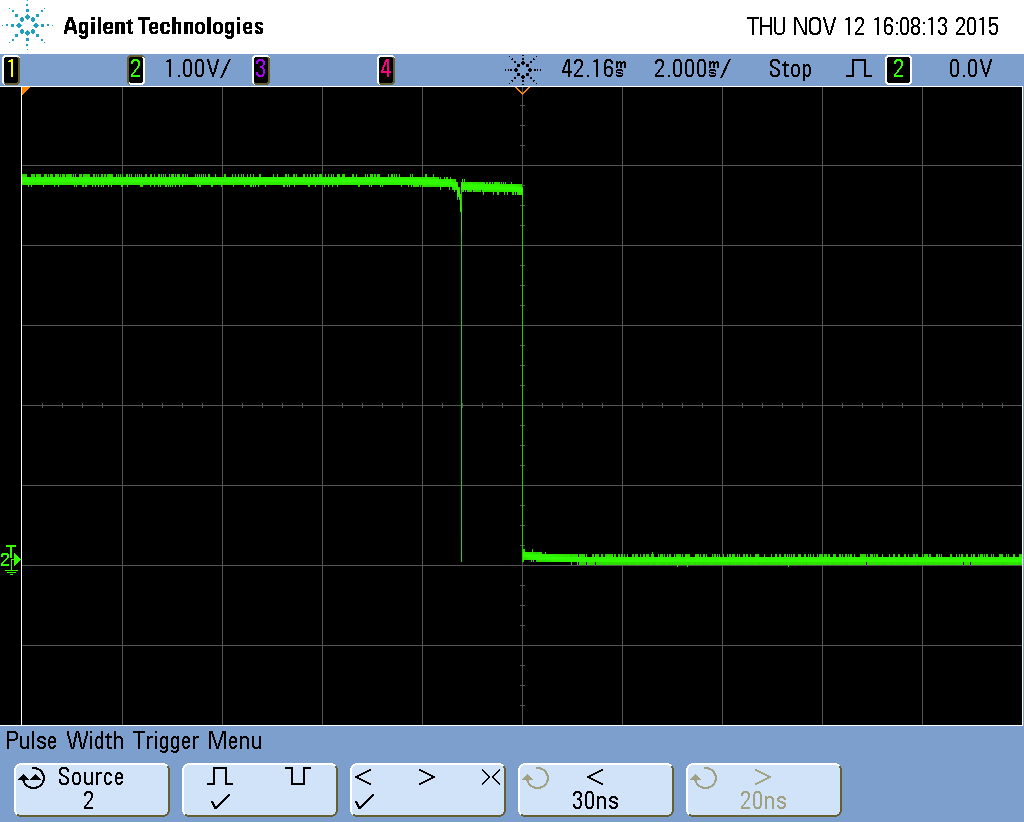
\includegraphics[width = \textwidth]{billeder/scope_14.png}
	\caption{Figuren viser et knaptryk, hvor der opstår debouncing.}\label{fig:withbounce}
\end{figure}

For at imødekomme  er der implementeret et debounce kredsløb (figur \ref{fig:antidebouncingcircuit}) med en inverting schmitt trigger. schmitt triggeren leverer en stabil høj og kapacitoren forhindre den lav ved kortvarig open circuit under knaptryk. 
\begin{figure}[H]
	\centering
	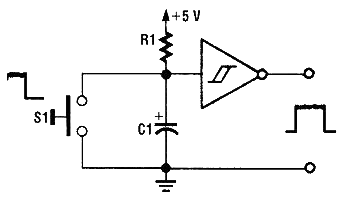
\includegraphics[width = 0.4\textwidth]{billeder/debounceSchematic.png}
	\caption{Anti debouncing kredsløb}\label{fig:antidebouncingcircuit}
\end{figure}

\begin{figure}[H]
	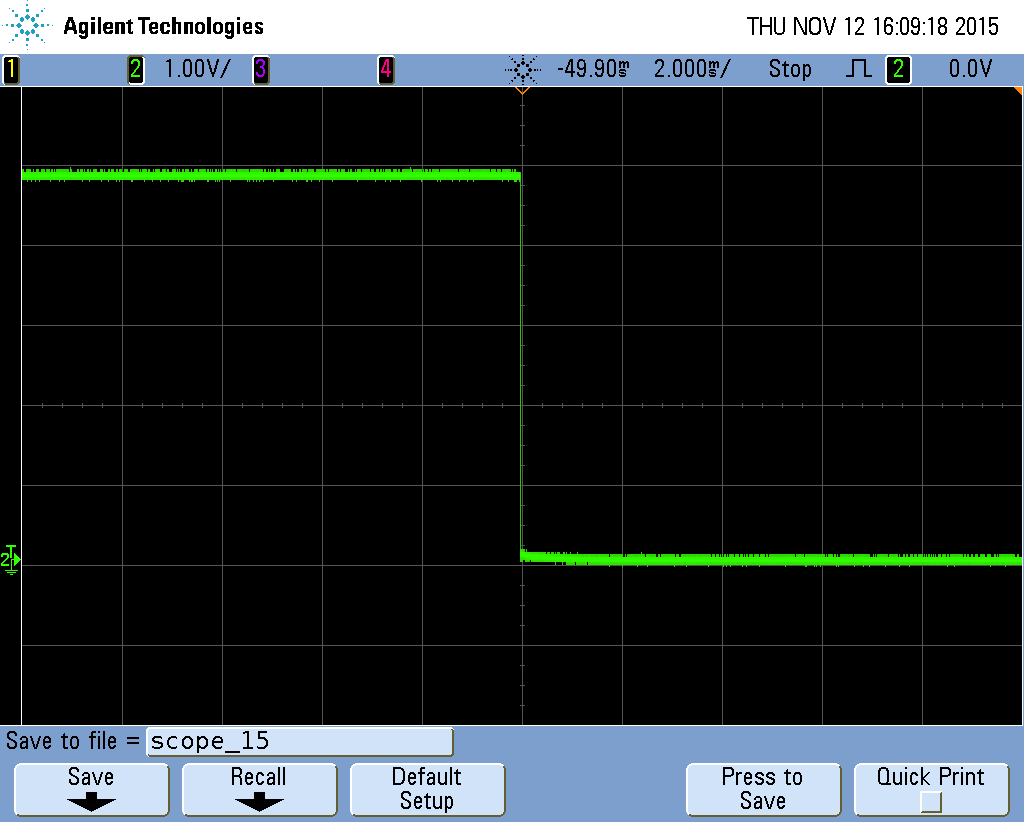
\includegraphics[width = \textwidth]{billeder/scope_15.png}
	\caption{Knaptryk hvor der er implementeret et anti debouncing kredsløb.}\label{fig:withoutbounce}
\end{figure}


\subsection{Filter}
Filtreringen af signalet er opdelt i isolering af manchet tryk og isolering af pulserende signal. På figur \ref{fig:filterschematics} ses opdelingen af signalet i to til ADCen. Dyberer forklaring af filterdesignet kan findes under afsnit \ref{title:filters} omkring filter design.

\begin{figure}[H]
	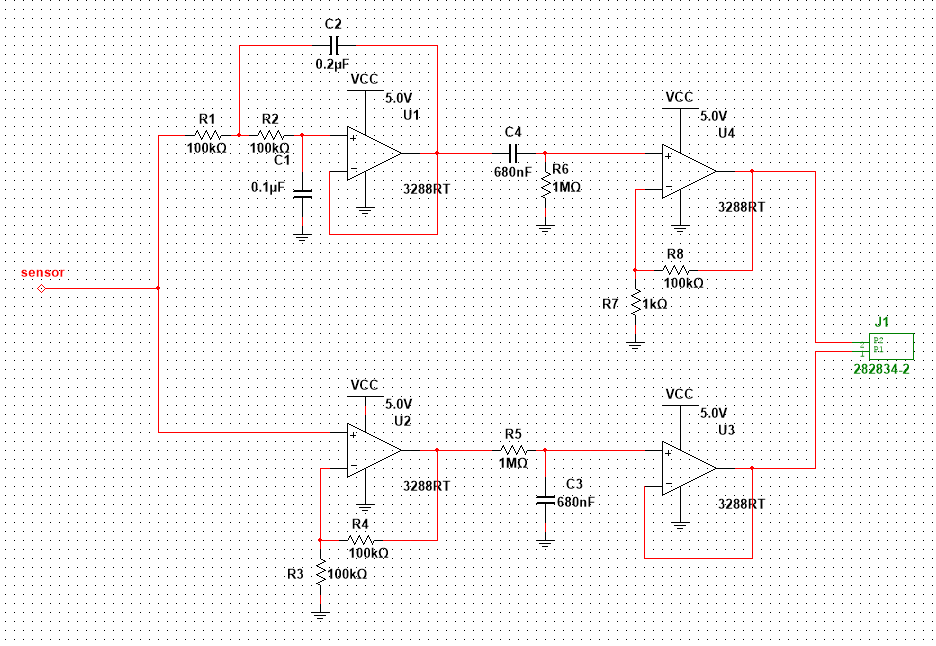
\includegraphics[width = \textwidth]{billeder/filterSchematics.png}
	\caption{Schematics over filter design}\label{fig:filterschematics}
\end{figure}